\section{Over all structure}

The work done on the project affected all the system to some degree. This section describes the key elements of the overall system when we started the semester, so it is easier to follow the work described throughout the report. 

The GIRAF content is divided into areas of responsibility, and hosted in several repositories on Gitlab. Figure \ref{fig:ProductStructure}

\begin{figure}[H]
    \begin{center}
        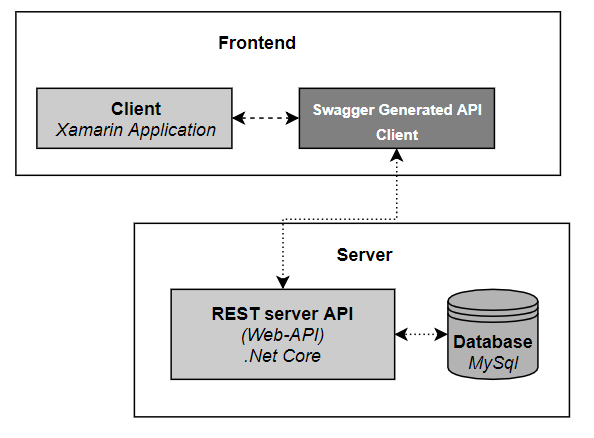
\includegraphics[width=0.95\textwidth]{figures/ProductStructure.png}
    \end{center}
    \caption{Overall structure of the GIRAF content}
    \label{fig:ProductStructure}
\end{figure}

\subsection{Frontend}
The Frontend contains the UI elements, called the client, and communication to the server. The client, which contains the UI material for the Weekplanner application uses the Xamarin framework. The framework makes it possible to make both Android and iOS applications. The application is structured with the MVVM pattern, where the models, the view, and the view models are separated. This means that the visual aspects are exclusively placed in the views, the business logic in the view models and the data objects that represent the data from the database in the models.

The communication between the client and the Web-API are done through an API client. In this report this is called the \gls{fapi}. The \gls{fapi} are auto generated by the software Swagger.

\subsection{Server}
The server contains both the database and the Web-api. The Web-api is build with the Rest principles. This means that it must uphold the following six guidelines\cite{REST}. is exposes endpoints to the frontend, and communicates with the database. 
All the server content are hosted in Docker containers and managed by the Kubernetes system. 
The server contains both the database and the Web-api. The Web-api is exposed through a rest API that communicates with the database. The Web-api is a .Net Core project, structured with the MVC pattern.



